\section{13-10-2014}
\subsection{Markov Chains 1.2}



\begin{defn}
We say that \emph{\(i\) leads to \(j\)} and write \(i\rightarrow j\) if
\[
\Bbb{P}_{i}(X_{n}=j\space \text{ for some }n\geq 0)>0.
\]
\end{defn}

\begin{defn}
We say \emph{\(i\) communicates with \(j\)} and write \(i\leftrightarrow j\) if both \(i\rightarrow j\) and \(j\rightarrow i\).
\end{defn}

\begin{thm}
For distinct states \(i\) and \(j\) the following are equivalent:

\begin{enumerate}
  \item \(i\rightarrow j\space \Longleftrightarrow \space \Bbb{P}_{i}(X_{n}=j\space \text{ for some }n\geq 0)>0\)
  \item \(p_{i_{1}i_{2}}p_{i_{2}i_{3}}\ldots p_{i_{n-1}i_{n}}>0\) for some states \(i_{1},\ldots ,i_{n}\) with \(i_{1}=i\) and \(i_{n}=j\)
  \item \(p_{ij}^n>0 \text{ for some } n\geq 0\)
\end{enumerate}

\end{thm}

\begin{proof}
Remember that
\[
p_{ij}^n=\Bbb{P}_{i}(X_{n}=j)=\sum _{i_{2},\ldots ,i_{n-1}}p_{ii_{2}}p_{i_{2}i_{3}}\ldots p_{i_{n-1}j}.
\]
From this everything follows.
\end{proof}

\begin{prop}
Show that \(i\rightarrow i\).
\end{prop}

\begin{proof}
\[
i\rightarrow i\space \Longleftrightarrow \space \space \Bbb{P}_{i}(X_{n}=i\space \text{ for some }n\geq 0)>0
\]

This follows, as \(\Bbb{P}_{i}(X_{0}=i)=1.\)
\end{proof}

\begin{defn}
The equivalence classes of the equivalence relations \(\leftrightarrow \) are called \emph{communicating classes}. We say that a class \(C\) is closed if
\[
i\in C, i\rightarrow j\space \Longrightarrow \space j\in C
\]
\end{defn}

\begin{defn}
A state \(i\) is \emph{absorbing} if \(\{i\}\) is a closed class.
\end{defn}

\begin{defn}
A chain or transition matrix \(P\) where \(I\) is a single class is called \emph{irreducible}.
\end{defn}

\begin{thm}[Example 1.2.2]
Find the communicating classes associated to the stochastic matrix
\begin{gather*}
P= \begin{pmatrix}\tfrac 12&\tfrac12&0&0&0&0\\
0&0&1&0&0&0 \\
\tfrac{1}{3}&0&0&\tfrac 13&\tfrac 13&0 \\
0&0&0&\tfrac{1}{2}&\tfrac{1}{2}&0 \\
0&0&0&0&0&1 \\
0&0&0&0&1&0
\end{pmatrix}
\end{gather*}
\end{thm}

\begin{proof}
The solution is obvious from the diagram. The classes being \(\{1,2,3\}, \{4\}\) and \(\{5,6\}\). With only \(\{5,6\}\) closed.

\begin{tikzpicture}
\SetGraphUnit{1}
\Vertices{circle}{1,2,3,4,5,6}
\Edges(1,2,3,1)
\Edges(3,4,5)
\Edges(3,5,6,5)
\end{tikzpicture}
\end{proof}
\begin{thm}[Exercise 1.2.1]
Identify the communicating classes of the following transition matrix:
\begin{gather*}
P=
\begin{pmatrix}\tfrac{1}{2}&0&0&0&\tfrac{1}{2} \\
0&\tfrac{1}{2}&0&\tfrac{1}{2}&0 \\
0&0&1&0&0\\
0&\tfrac{1}{4}&\tfrac{1}{4}&\tfrac{1}{4}&\tfrac{1}{4} \\
\tfrac{1}{2}& 0&0&0&\tfrac{1}{2}\end{pmatrix}
\end{gather*}
\end{thm}

The solution is obvious from the diagram. The classes being \(\{1,5\}, \{2,4\}\) and \(\{3\}\). With  \(\{1,5\}\) closed and \(\{3\}\) absorbing.
\begin{tikzpicture}
\SetGraphUnit{1}
\Vertices{circle}{1,2,3,4,5}
\Edges(1,5,1)
\Edges(4,2,4,5)
\Edges(4,3)
\end{tikzpicture}

\subsection{Markov Chains 1.3}
\begin{defn}
Let \(X_{n}\) be a Markov chain with transition matrix \(P\). The \emph{hitting time} of a subset \(A\) of \(I\) is the random variable
\[
H^A: \Omega \rightarrow \{0,1,2,\ldots ,\infty \}
\]
given by
\[
H^A(\omega )=\inf\{n\geq 0 :X_{n}(\omega )\in A\}
\]
where we agree that the infimum of the empty set \(\varnothing \) is \(\infty \). The probability starting from \(i\) that \((X_{n})_{n\geq 0}\) ever hits \(A\) is then
\[
h_{i}^A=\Bbb{P}_{i}(H^A<\infty ).
\]
When \(A\) is a closed class, \(h_{i}^A\) is called the \emph{absorption probability}. The mean time taken for \(X_{n}\) to reach \(A\) is given by
\[
k_{i}^A=E_{i}(H^A)=\sum _{n<\infty }n\Bbb{P}(H^A=n)+\infty \Bbb{P}(H^A=\infty ).
\]
We shall often write less formally
\[
h_{i}^A=\Bbb{P}_{i}(\text{hit }A) \qquad k_{i}^A=E_{i}(\text{time to hit }A).
\]
\end{defn}

\begin{thm}[Example 1.3.1]
Consider the chain with following diagram:

\begin{tikzpicture}
\SetGraphUnit{2}
\Vertices{line}{1,2,3,4}
\Edge[label=\tiny$\tfrac12$](2)(1)
\Edge[label=\tiny$\tfrac12$](3)(4)
\tikzset{EdgeStyle/.append style = {bend left}}
\Edge[label=\tiny$\tfrac12$](2)(3)
\Edge[label=\tiny$\tfrac12$](3)(2)
\end{tikzpicture}

\begin{enumerate}
  \item Starting from 2, what is the probability of absorption in \(4\)?
  \item How long does it take until the chain is absorbed in \(1\) or \(4\) ?
\end{enumerate}
\end{thm}


\begin{proof}
\begin{enumerate}
  \item Note that \(A=\{4\}\) is a closed class. The aborption probability is defined as
\[
h_{i}:=h_{i}^{\{4\}}=\Bbb{P}_{i}(\text{hit } 4).
\]
We have
\begin{align*}
h_{1}&=0 \\
h_{4}&=1 \\
h_{2}&=\tfrac{1}{2}h_{1}+\tfrac{1}{2}h_{3} = \tfrac{1}{2}h_{3} \\
h_{3}&= \tfrac{1}{2}h_{2}+\tfrac{1}{2}h_{4}=\tfrac{1}{2}h_{2}+\tfrac{1}{2}
\end{align*}
Hence
\begin{align*}
&h_{2}=\tfrac{1}{4}h_{2}+\tfrac{1}{4} \\
\Longrightarrow \  &\tfrac{3}{4}h_{2} = \tfrac{1}{4} \\
\Longrightarrow \  &h_{2}=\tfrac{1}{3}
\end{align*}
  \item We need to compute
\[
k_{2}=k_{2}^{\{1,4\}}=E_{2}(\text{time to hit } \{1,4\}).
\]
We have
\begin{gather*}
k_{1}=0 \\
k_{4} = 0 \\
k_{2} = 1+\tfrac{1}{2}k_{3} \\
k_{3} = 1+ \tfrac{1}{2} k_{2}
\end{gather*}
Hence
\begin{align*}
&k_{2} = \tfrac{3}{2} + \tfrac{1}{4} k_{2} \\
\Longrightarrow \ \space &\tfrac{3}{4} k_{2}= \tfrac{3}{2} \\
\Longrightarrow \ \space &k_{2}=2
\end{align*}
\end{enumerate}
\end{proof}

\begin{thm}[Theorem 1.3.2]
The vector of hitting probabilities \(h^A=(h_{i}^A:i\in I)\) is the minimal non-negative solution to the system
\begin{align*}
\begin{cases}h_{i}^A=1 &\text{for}\space i\in A \\ h_{i}^A=\sum _{j\in I}p_{ij}h_{j}^A &\text{for }i\not\in A.\end{cases}
\end{align*}
Minimality means that if \(x=(x_{i}:i\in I)\) is another solution with \(x_{i}\geq 0\) for all \(i\), then \(x_{i}\geq h_{i}\) for all \(i\).
\end{thm}

\begin{thm}[Example 1.3.1(continued)]
Use theorem 1.3.2 to compute \(h_{2}\) again.
\end{thm}

\begin{proof}
The vector of hitting probabilities \(h^{\{4\}}=\Big(h_{1}^{\{4\}},h_{2}^{\{4\}},h_{3}^{\{4\}},h_{4}^{\{4\}}\Big)\) is the minimal non-negative solution to the system
\begin{align*}
&h_{1}^{\{4\}}=\sum _{j\in I}p_{ij}h_{j}^{\{4\}}=h_{1}^{\{4\}}\\
&h_{2}^{\{4\}}=\sum _{j\in I}p_{ij}h_{j}^{\{4\}}=\tfrac{1}{2}h_{1}^{\{4\}}+\tfrac{1}{2}h_{3}^{\{4\}}\\
&h_{3}^{\{4\}}=\sum _{j\in I}p_{ij}h_{j}^{\{4\}}=\tfrac{1}{2}h_{2}^{\{4\}}+\tfrac{1}{2}h_{4}^{\{4\}}\\
&h_{4}^{\{4\}}=1
\end{align*}
The minimality condition gives, that \(h_{1}^{\{4\}}=0\). So that <br />
\begin{align*}
&h_{2}^{\{4\}}=\tfrac{1}{2}h_{3}^{\{4\}}\\
&h_{3}^{\{4\}}=\tfrac{1}{2}h_{2}^{\{4\}}+\tfrac{1}{2}
\end{align*}
which gives:
\begin{align*}
&h_{2}^{\{4\}}=\tfrac{1}{4}h_{2}^{\{4\}}+\tfrac{1}{4}\space \Longrightarrow \space h_{2}^{\{4\}}=\tfrac{1}{3}\\
&h_{3}^{\{4\}}=\tfrac{1}{4}h_{3}^{\{4\}}+\tfrac{1}{2}\space \Longrightarrow \space h_{3}^{\{4\}}=\tfrac{2}{3}
\end{align*}
\end{proof}

\begin{thm}
Consider a recurrence relation of the form
\[
ax_{n+1}+bx_{n}+cx_{n-1}=0 \qquad a,c\neq 0.
\]
Let \(\alpha ,\beta \) be the roots of the quadratic equation
\[
ax^2+bx+c.
\]
Then the general soltuions is given by
\begin{align*}
x_{n}=\begin{cases}A\alpha ^n+B\beta ^n &\text{if }\alpha \neq \beta \\ (A+nB)\alpha ^n &\text{if }\alpha =\beta \end{cases}
\end{align*}
\end{thm}

\begin{prop}
Give a general solution for the recurrence relation
\begin{align*}
h_{0}&=1 \\
h_{i}&=ph_{i+1} +qh_{i-1}
\end{align*}
\end{prop}

\begin{proof}
Note that we have
$-ph_{i+1}+h_{i}-qh_{i-1}=0$. Consider
\[
-px^2+x-1+p=0
\]

We have the roots \(\alpha =1,\beta =\tfrac{q}{p}\). If \(q\neq p\), this gives
\[
h_{i}=A\alpha ^i+B\beta ^i=A+B\Big(\frac{q}{p}\Big)^i.
\]
And if \(p=q\), then \(\alpha =\beta =1,\) and we have
\[
h_{i}=A\alpha ^i+B\beta ^i=A+iB
\]
\(\)
\end{proof}




\begin{thm}[Example 1.3.3]
Consider the Markov chain with diagram

\begin{tikzpicture}
\SetGraphUnit{2}
\Vertices{line}{0,1}
\Vertex[Math,L=\ldots,x=4,y=0] {dots}
\Vertices[x=6,y=0]{line}{i,i+1}
\Vertex[Math,L=\ldots,x=10,y=0] {dots2}
\Edge[label=q](1)(0)
\tikzset{EdgeStyle/.append style = {bend left}}
\Edge[label=p](1)(dots)
\Edge[label=q](dots)(1)
\Edge[label=p](dots)(i)
\Edge[label=q](i)(dots)
\Edge[label=p](i)(i+1)
\Edge[label=q](i+1)(i)
\Edge[label=p](i+1)(dots2)
\Edge[label=q](dots2)(i+1)
\end{tikzpicture}

where \(0<p=1-q<1\). What is \(h_{i}=\Bbb{P}_{i}(\text{hit } 0)\)?
\end{thm}

\begin{proof}
We know that \(h\) is the minimal non-negative solution to
\begin{align*}
h_{0}&=1 \\
h_{i}&=ph_{i+1} +qh_{i-1}
\end{align*}

We consider some cases: 
\begin{itemize}
  \item Suppose \(p=q\), then we have
\[
h_{i}=A\alpha ^i+B\beta ^i=A+iB
\]
and as $0\leq h_{i}\leq 1$ is a probability, we must have $B=0$. We then have
\[
h_{i}=A,
\]
and as \(h_{0}=1,\) we must have $h_{i}=1$.
  \item Suppose $p\neq q$, we then have
\[
h_{i}=A\alpha ^i+B\beta ^i=A+B\Big(\frac{q}{p}\Big)^i.
\]
If \(\frac{q}{p}>1,\) then we must set $B=0$ again.
  \item Suppose \(\frac{q}{p}<1\). We have that $h_{0}=1$, and therefore \(A+B=1.\) Hence:
\[
h_{i}=(\tfrac{q}{p})^i+A\Big(1-(\tfrac{q}{p})^i\Big)
\]
So the minimal non-negative solutions is \(h_{i}=(q/p)^i\).
\end{itemize}
\end{proof}



\begin{thm}[Example 1.3.4]
Consider the Markov chain with diagram

\begin{tikzpicture}
\SetGraphUnit{2}
\Vertices{line}{0,1}
\Vertex[Math,L=\ldots,x=4,y=0] {dots}
\Vertices[x=6,y=0]{line}{i,i+1}
\Vertex[Math,L=\ldots,x=10,y=0] {dots2}
\Edge[label=$q_1$](1)(0)
\tikzset{EdgeStyle/.append style = {bend left}}
\Edge[label=$p_1$](1)(dots)
\Edge[label=$q_2$](dots)(1)
\Edge[label=$p_{i-1}$](dots)(i)
\Edge[label=$q_i$](i)(dots)
\Edge[label=$p_i$](i)(i+1)
\Edge[label=$q_{i+1}$](i+1)(i)
\Edge[label=$p_{i+1}$](i+1)(dots2)
\Edge[label=$q_{i+2}$](dots2)(i+1)
\end{tikzpicture}

where for \(i=1,2,\ldots ,\) we have $0<p_{i}=1-q_{i}<1$. As in the preceding example, $0$ is the absorbing state, and we wish to calculate the absorption probability starting form $i$.
\end{thm}

\begin{proof}
Consider the system of equations
\begin{align*}
h_{0}&=1 \\
h_{i}&=p_{i}h_{i+1}+q_{i}h_{i-1} \qquad\text{for }i=1,2,\ldots 
\end{align*}
Consider
\begin{align*}
u_{i}:&=h_{i-1}-h_{i},
\end{align*}
then
\begin{align*}
&p_{i}u_{i+1}=p_{i}h_{i}-p_{i}h_{i+1}\\
&q_{i}u_{i}=q_{i}h_{i-1}-q_{i}h_{i} \\ \\
\Longrightarrow \  &q_{i}u_{i}-p_{i}u_{i+1}=h_{i}-q_{i}h_{i}-p_{i}h_{i}=0
\end{align*}
Therefore \(p_{i}u_{i+1}=q_{i}u_{i}\) and we have
\[
u_{i+1}=\Big(\frac{q_{i}}{p_{i}}\Big)u_{i}=\prod _{j=1}^i \frac{q_{i}}{p_{i}}u_{1}=\gamma _{1}u_{1}
\]
We also have
\[
u_{1}+\ldots +u_{i}=h_{0}-h_{i}
\]
so
\[
h_{i}=h_{0}-(u_{1}+\ldots +u_{i})=1-u_{1}(\gamma _{0}+\ldots +y_{n-1}).
\]
At this point \(A\) remains to be determined. In the case that \(\sum _{i=0}^\infty \gamma _{i}=\infty \), we must have \(A=0.\) In the other case, we can't take \(A<0,\) but we can take $A>0$ so long as
\[
h_{i}=1-A\sum _{i=0}^{i-1}\gamma _{i} \geq 0.
\]
Which means that
\[
A\leq (\sum _{i=0}^{i-1}\gamma _{i})^{-1}
\]
but still as big as possible. So we get
\[
A=(\sum _{i=0}^{\infty }\gamma _{i})^{-1}.
\]
And therefore
\[
h_{i}=\frac{\sum _{j=i}^{\infty }\gamma _{j}}{\sum _{j=0}^{\infty }\gamma _{j} }
\]
\end{proof}

\begin{thm}[Theorem 1.3.5]
The vector of mean hitting times \(k^A=(k^A:i\in I)\) is the minimal non-negative solution to the system of linear equations
\begin{align*}
\begin{cases}k_{i}^A=0 &\text{for }i\in A \\ k_{i}^A=1+\sum _{j\not\in A}p_{ij}k_{j}^A &\text{for }\not\in A\end{cases}
\end{align*}
\end{thm}

